\subsection{Per-Operator Evaluation}

% We have performed simulation-based validation to check the correctness of all the compiler IR to accelerator mappings for our target accelerators, with verification tasks of the VT1, VT2 and VT3 in Figure \ref{fig.mapping}. 
% During the simulation, the models from two sides of the mapping are given the same input tensor data, and we measure the relative errors between the results from two sides. 

% 1. what we are checking
% 2. describe the results in the table
% 3. what do the results tell us

%Although comparing the accuracy of individual operators
Having now evaluated \cref{thesis:devtime}
  and \cref{thesis:optimizations},
  we will evaluate \cref{thesis:correctness}.
We do so by demonstrating how \g, via \TLA,
  enables testing of accelerators.
We begin by evaluating single operators. 
Although evaluating individual operators
  does not suffice to characterize
  how an accelerator performs on a full application,
  it is a basic first step
  and provides 
  insights on the identified acceleration opportunities.
  %validation of 
  %the given compiler IR--accelerator mappings.
  %it provides (i) a basic first step toward end-to-end
  %testing and (ii) validation
  %of the given compiler IR-accelerator mappings.
%Due to auto-generated ILA simulators, this 
  % is readily enabled by the {\TLA} methodology.
%The auto-generated ILA simulators
  % readily enable this in the {\TLA} methodology.
Here, we discuss both functional validation and performance evaluation at the operator level.

%Modern accelerators often adopt custom numerics for achieving better power-performance efficiency.
%
%For example, in our cases, FlexASR and HLSCNN use the AdaptivFloat and 8/16-bit fixed point data types, respectively.
%
%This means checking the IR-accelerator mappings must account for the numerical differences.
%
%%To separate the effect of numerics and focus on the definition of operations, we use abstract data types to formally verify the equivalence
%(demonstrated through a proof-of-concept case study).
%
%On the other hand, 
%%In addition, to precisely capture the numerical differences, we use simulation to compare accelerator executions (using an ILA simulator) against the IR semantics (using an IR interpreter).

%\para{Simulation-Based Validation}

% Recognize the deviation due to custom numerics.
% How: the setup
% Summarize: op-level accuracy is relatively good

% Among the three verification tasks, we see negligible mismatch in VT1, which is from the rounding errors of floating-point numerics. 
% In VT3, we have an exact match between accelerator ILA and accelerator implementation simulation results, despite the modeled accelerator implementations may have their customized numerical representation (e.g., customized 8-bit floating point system in FlexASR \cite{tambe2020algorithm} and 8-bit fixed point representation in HLSCNN). 
% This is because the generated simulator from accelerator ILA supports custom numeric computation from the accelerators' original implementation as "plug-ins" to fully model the behaviors of the accelerator in both computation definition and numerical representation.
% Based on VT1 and VT3, we can check the mapping correctness by performing VT2. 

\subsubsection{Functional Validation}

\begin{table}
\caption{
\textbf{
Simulation-based validation results for checking {\mapping}s.
}
% We measure the relative errors of VT2 using tensors' Frobenius Norm as:
% $Error = \norm{Out_{ref} - Out_{acc}}_F / \norm{Out_{ref}}_F$. 
% We measure the relative errors of the accelerator program fragment simulation results against the compiler simulation results on host processor with the following function using tensors' Frobenius Norm:
% $Error = \frac{\norm{Out_{ref} - Out_{acc}}_F}{\norm{Out_{ref}}_F} * 100\%$. 
The average relative error (Avg. Err.) and the standard deviation (Std. Dev.) of errors are measured 
%for simulations 
over 100 test inputs. % with randomly generated inputs.
% See Table \hl{TODO} in the Appendix for the complete validation results of all IR-accelerator mappings.
For VTA, 
%we compared GEMM, add, and max operations; 
there was no error because the host supports 
8-bit integer operations.
%these operations in 8-bit integer.
}
\label{tab.layer-sim}
\centering
\begin{small}
\begin{tabular}{|c|l|l|r|r|}
\hline
  & Accel. & Operation & Avg.Err. & Std.Dev.  \\
  \hline \hline
  1 & VTA & All ops & 0.00\% & 0.00\% \\ % \hline
  2 & HLSCNN & Conv2D & 1.78\% & 0.16\% \\ % \hline
  3 & FlexASR & LinearLayer & 0.84\% & 0.29\% \\ % \hline
  4 & FlexASR & LSTM & 1.21\% & 0.19\% \\ % \hline 
  5 & FlexASR & LayerNorm & 0.27\% & 0.20\% \\ % \hline
  6 & FlexASR & MaxPool & 0.00\% & 0.0\% \\ % \hline
  7 & FlexASR & MeanPool & 1.79\% & 0.28\% \\ % \hline
  8 & FlexASR & Attention & 4.22\% & 0.09\% \\ 
\hline
\end{tabular}
\end{small}
\end{table}

The {\TLA} methodology readily enables operator-level validation through auto-generated ILA simulators.
%For operator-level testing,
%compiler IR-accelerator mappings through simulation, 
In our experiments, we 
%generated 100 random test inputs and 
compared the outputs of the accelerator ILA simulator and those of TVM's runtime on host.
%
The accelerator ILA simulators precisely model the data types used by the accelerators.
%
%\hl{Specifically, VTA, HLSCNN, and FlexASR use 8-bit integer, mixed 8/16-bit fixed point, and AdaptivFloat, respectively.}
%
%For the reference results (TVM's runtime), we use 8-bit integer, 32-bit floating point, and 32-bit floating point when checking VTA, HLSCNN, and FlexASR operations, respectively. These are the closest host processor data types to those used by the accelerators. 
For the reference results (TVM's runtime), we use 8-bit integer for comparing against VTA and 32-bit floating point for the other accelerators, as these are the closest host processor data types to those used by the accelerators. 
%
We measure the relative errors by using the standard Frobenius Norm~\cite{lapack} for the tensors based on the reference and accelerator generated output values as follows:
%$Error = \norm{Out_{ref} - Out_{acc}}_F / \norm{Out_{ref}}_F$.
$Error = \| Out_{ref} - Out_{acc} \|_F / \| Out_{ref} \|_F$.
\iffalse
\[
Error = \frac{\norm{Out_{ref} - Out_{acc}}_F}{\norm{Out_{ref}}_F} * 100\% 
\]
\fi
% Here, $Out_{ref}$ and $Out_{acc}$ are the IR reference and accelerator outputs, respectively.

We validated all types of operators supported by the target accelerators.
Table~\ref{tab.layer-sim} shows a representative subset of the validation results: four {\mapping}s (Rows~1-4) that are used in the full application compilation (Table~\ref{tab.compilation}) and four additional mappings for non-trivial operations (Rows~5-8).
%We omitted validation results of other mappings, e.g., for trivial operations \textit{add} and \textit{max}. \hl{SM: Are these the only results omitted?}
% See Table \hl{TODO} in the Appendix for complete validation results of all IR-accelerator mappings.
% Table~\ref{tab.layer-sim} shows the validation results. 
% The top four compiler IR-accelerator mappings are used in our end-to-end compilation experiments. 
% We also perform simulation validation for all the other mappings, but some of them are trivial operations, such as \textit{add} or \textit{max} in VTA operations. 
% Here we show four more non-trivial mappings' validation results.
%
%Columns~1 and~2 indicate the accelerator and the supported operation for each compiler IR-accelerator mapping, respectively.
%
%Columns~3 and~4 report the average relative error and the standard deviation, respectively, over the 100 test inputs.
%
Note that some mappings introduce no numerical differences; e.g., the TVM runtime supports 8-bit integer execution, so the results for VTA match perfectly.
%For mappings that are not affected by numerical differences, e.g., the VTA-supported GEMM, we see exact matches in the results.
%
For other mappings, we see deviations caused by the custom numerics, especially for complex operators such as the attention operator on FlexASR.  
% yes
%\hl{AG: comment on deviations? does this mean we should watch end-to-end more carefully?}
Such deviations should be carefully assessed
  in the context of application-level validation,
  as even small deviations could accumulate and affect the final accuracy.

% Table \ref{tab.layer-sim} shows the simulation results for compiler IR-accelerator mappings of the three different accelerators.
% The range and distribution of the testing inputs are determined based on the target application of the accelerators and the input values are quantized.
% VTA is using standard 8-bit integer datatype and shows an exact matched with the Relay IR program fragment results which also using the same 8-bit integer for computation. 
% However, since there is no support for the customized floating-point or fixed point numerics used in HLSCNN and FlexASR, the Relay IR program for these mappings simulated with standard 32-bit floating-point representation. 
% Among these mappings, we only observe small relative errors, which shows the correctness of the mappings with acceptable deviation with the custom numerical representation in the accelerators.

\subsubsection{Performance Evaluation}

%The {\TLA} methodology enables performance evaluation on the operators that will be accelerated in the full application compilation.
%--- allowing comparing the precise number of exact offloaded host operators against the invoked accelerator operators.
%In our experiments, we 
We also evaluated the performance gain of offloading operations from the host to accelerators 
%(identified as reported in Table~\ref{tab.compilation}) 
using cycle counts as the performance metric, since we did not have clock frequencies for an SoC containing the host and accelerators.
%\footnote{
%Precise performance modeling depends on various factors, e.g., processing technology node, that may not yet be available for prototype accelerators, like in HLSCNN and VTA.
%We chose cycle count as the appropriate metric for (micro-)architectural design evaluation.
%}
%\aarti{We used this metric since clock rates might vary and are, in fact, a design consideration.}
For accelerators, we derived the cycle counts based on their cycle-accurate models
(VTA's Chisel model
%TSIM for VTA
and FlexASR's and HLSCNN's SystemC models).
%RTL implementation (FlexASR and HLSCNN)
%\yl{Right now FlexASR and HLSCNN performance models are based on their cycle-accurate SystemC simulation model}
%or the cycle-accurate Chisel-generated simulator (VTA).
%We measured average cycle counts of operators executed in TVM's runtime on host (EPYC0000) over 2000 random inputs.
For the host, we measured averaged cycle counts (1000 random inputs) in TVM's runtime
%, averaging over 2000 random inputs 
on one pinned EPYC-7532 core.

% I don't think we need this for dissertation.
\begin{figure}
  \centering
  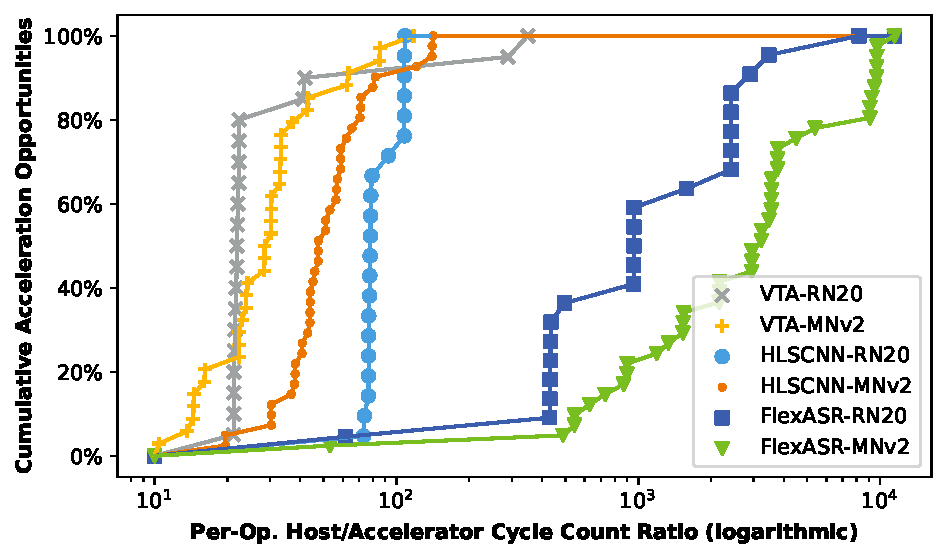
\includegraphics[width=.65\linewidth]{3la/Figures/performance.pdf}
  \caption{
\textbf{
Cumulative distribution of per-operator performance gains of all identified acceleration opportunities} in ResNet-20 (RN20) and MobileNet-V2 (MNv2) on the three accelerators.
%VTA, HLSCNN, and FlexASR.
Each point represents an operation offloaded from the host to the accelerator (as identified by flexible matching, Table~\ref{tab.compilation}).
The $x$-axis shows the host-to-accelerator cycle count ratio of each offloaded operation 
%(the bigger the better); 
and the $y$-axis shows the cumulative distribution of offloaded operations. Points and plots more to the right are better; e.g., coarse-grained operators, supported with higher parallelism in FlexASR, offer greater speedup compared to the fine-grained operators in VTA. %\sm{Change Accumulative in figure to Cumulative.}
%the y-axis accumulates toward all identified acceleration opportunities in an application.
%The measurement is done on 2000 random inputs from the CIFAR-10 dataset~\cite{cifar10}. \yl{The test inputs are not from CIFAR-10 dataset. It is just a random input with the same shape to the layer input in the applications}
}
  \label{fig.performance}
% \Description{}
\end{figure}

Fig.~\ref{fig.performance} shows the performance gains (ratio of host to accelerator cycles) of all identified acceleration opportunities in ResNet-20 and MobileNet-V2 when operations are offloaded from the host to VTA, HLSCNN, and FlexASR, respectively. 
%Figure~\ref{fig.performance} shows the cycle count ratios of all offloaded operations (from the host to the accelerator) in ResNet-20 and MobileNet-V2 when compiled to VTA, HLSCNN, and FlexASR.
%the three accelerators.
%Each point represents an operation offloaded from the host to the accelerator.
Overall, as expected, all offloads resulted in performance gains relative to the host; we also see that accelerators providing coarser-grained operators (e.g., FlexASR), supported with higher parallelism, achieve higher performance gain per operator compared to finer-grained accelerators like VTA. %\sslyu{Is this really something we should highlight? We don't discuss performance gains of coarse-grained vs fine-grained accelerators in the intro; our point is just that we gain performance compared to the host, which is what we're aiming for.}
%\aarti{
%Although the graph does not compare operator attributes, such as convolution strides, such per-operator performance evaluation can also provide additional insights on how these properties affect the performance of offloaded operators. 
%such as how the Conv2D operator performs under different stride attributes and \texttt{im2col} matrix dimensions.
%This could be useful in future work for performance optimization.
%} 
%\sslyu{Are we reporting any data to suggest that conclusion? We shouldn't say this if we don't. Otherwise, we could say that our methodology for getting the cycle counts could be used for assessing these issues.}
%We also find such per-operator performance evaluation insightful.
%Take VTA for example, {\TLA} provides a convenient way to analyze, within a real application, how the Conv2D operator performs under different convolution stride attributes and \texttt{im2col} matrix dimensions.
% From the operator-level performance analysis, we also see that VTA is not always good.
%We also found that the same Conv2D operator of VTA performs better when the convolution strides attributes align well with the \texttt{im2col} matrix dimensions---up to 10x difference in performance gain.
% \yl{VTA performs better stride attributes in the Conv2D are larger than 1. The reason is that larger strides would reduce the matrix size for matrix multiplications after doing im2col.}
%By measuring the performance of both running 2D Convolutions layers and running corresponding Dense matrix multiplications obtained from the \texttt{im2col} optimization, we found that VTA does not always gain performance from the optimization unless the strides attributes of the convolution layer keep the \texttt{im2col} matrix dimensions small enough. 
%(\yl{Not sure we should put the comparison between our codegen with original VTA codegen in here though. We are not using the original VTA codegen for Conv2D in our experiment. Also this comparison deviates a little from the other comparisons between acc. and host CPU.})
%(\mh{See numbers in the table and conv2d configurations of those layers}) 
%Under certain settings, the optimization brings up to 4x speed-up while in some other cases, it makes 2x worse performance compared with the baseline operator.
%Such per-operator performance evaluation provides insights on the identified acceleration opportunities in the full application compilation and is critical to more thorough performance optimization.
%It is critical to more thorough performance optimization.
%In this way, enabling per-operator performance evaluation would help accelerator users identify the right place to apply such optimizations.
%This study demonstrates that the {\TLA} methodology enables performance evaluation at the operator level, providing insights on how the identified acceleration opportunities perform in a full application.
%This is critical to future performance optimization.


\iffalse
\para{Proof-Based Formal Verification}
\label{sec:fv}
%%% there are differences, likely due to numerics, and we want to check that using abstract data types
%%% summrize: we can formally prove small scale op-level mappings

%%% As described earlier in Section~\ref{sec.method.verif}, verification of the full flow includes task VT2, which verifies equivalence of the ILA program fragment on the compiler side with that on the accelerator side. 
%%% This section describes a proof-of-concept study on the  Relay and FlexASR fragments for the temporal max-pooling application (see Appendix for the ILA code).

%%% In formally verifying the mappings, we use abstract data types to separate the effect of custom numerics.

The key challenges in formally verifying mappings between fragments that represent DL computations include:
\begin{inlinelist}
  \item handling nested loops, for both compiler side and accelerator side, that iterate through tensor elements, and
  \item relating tensor variables between the two sides which may employ various tiling mechanisms.%, and
%   \item handling custom numerics.
\end{inlinelist}
%
%%% Although the code of each ILA fragment is small, there are challenges due to:
%%% \begin{itemize}
%%%     \item multiple nested loops: 4 levels of nesting on Relay side, 3 on FlexASR side.
%%%     \item \emph{aligning} the nested loops for checking equivalence
%%%     \item mapping the input matrix to a special customized tiling provided by FlexASR~\cite{tambe20219}. \footnote{\hl{We ignore the FlexASR numerics accuracy in this study.}}
%%% \end{itemize} 
%
As a proof-of-concept study, we considered the Relay and FlexASR fragments for the FlexASR MaxPool IR-accelerator mapping. These fragments both have 
3+ nested loops, and the relation between the two fragments must account for a special customized tiling provided by 
FlexASR~\cite{tambe20219}.
For this study, we considered %
equivalence of the fragments over %
fixed-sized tensors with symbolic data,\footnote{Formally modeling custom numerics is left to future work.} and implemented verification using two methods:
\begin{inlinelist}
  \item bounded model checking (BMC)~\cite{biere2003bounded}, and 
  \item program verification using constrained Horn clauses (CHCs)~\cite{komuravelli2016smt}. 
\end{inlinelist}
%
The BMC-based method unrolls all the loops in both fragments, which is straightforward but may fail to scale for large-sized tensors.
%
The CHC-based method is given a product program of the two fragments and uses \emph{relational} loop invariants, i.e., formulas that relate the two fragments at intermediate loop boundaries (details are beyond the scope of this paper). 
%
This avoids loop unrolling and can handle large tensors. 
Both methods use Z3~\cite{de2008z3} as the underlying SMT solver.

% In our case study, we provided invariants that capture the customized tiling of FlexASR for fixed-sized matrices. 
% (In future work, we will consider automatic inference of such loop invariants.) 

While ILAng directly supports BMC, we manually created CHCs for the CHC-based method.
%for a 2D MaxPool operation in FlexASR. 
We also supplied the relational invariants that capture the customized tiling of FlexASR.
%
In future work, we plan to automate CHC generation, which will allow formal verification of other IR-accelerator mappings used in this paper.
%
Table~\ref{tab.verif-formal} shows the results for this case study for various dimensions of the 2D input matrix (Column~1), with runtimes of the BMC-based and CHC-based verification methods in Columns~2 and~3, respectively. 
%
The BMC-based method was able to verify equivalence of mappings with small-sized matrices, but timed out (with a 3-hour time limit) on the $16 \times 64$ matrix that was used for simulation-based validation. % (based on the available accelerator testcases).
%
In contrast, the CHC-based method was faster than BMC and successfully verified mappings with larger matrices. These results are encouraging and demonstrate how the \TLA methodology enables formal verification of key steps in the compilation flow. 
\fi
%
% Our results for both methods are reported in Table~\ref{tab.verif-formal}, for verification runtime on input matrices of various dimensions.
%TODO: add interpretation
